% Preamble
\documentclass[12pt, a4paper]{report}

% Packages
\usepackage{titlesec,graphicx,tabularx,amsmath,indentfirst,multirow}
\usepackage[T2A] {fontenc}
\usepackage[russian]{babel}
\usepackage[utf8x] {inputenc}
\usepackage[top=2cm, bottom=2cm, left=1.5cm, right=1cm]{geometry}

\titleformat{\section}
{\Large\bfseries} % format
{}                % label
{0pt}             % sep
{\Large}          % before-code

\begin{document}
    \begin{footnotesize}
        \textit{\mbox{Федеральное государственное бюджетное образовательное учреджение высшего профессионального образования}}\\
    \end{footnotesize}

    \begin{tabular}{c c}
        \multirow{4}{*}{
\includegraphics[scale = 0.03]{mgtu.png}}
        & \\
        & \footnotesize\textit{\textbf{\guillemotleftМосковский государственный технический университет имени Н.Э. Баумана\guillemotright}}\\
        & \\
        & \textit{\textbf{(МГТУ им. Н.Э. Баумана)}}\\
        & \\
        & \\
        & \\
        \hline\\
    \end{tabular}

    ФАКУЛЬТЕТ \guillemotleftИнформатика и системы управления\guillemotright\\

    КАФЕДРА \guillemotleft Компьютерные системы и сети\guillemotright\\

    \vfill

    \begin{center}

        \textbf{Отчет}\\
        \bigskip
        \textbf{по домашнему заданию №1}\\
        \bigskip
        \textbf{Дисциплина: Электротехника}\\
        \bigskip
        \textbf{Название лабораторной работы: Анализ линейной электрической цепи\\ постоянного тока.}\\
        \bigskip\bigskip
        \textbf{Вариант 25.}\\

        \vfill

        \begin{tabularx}{\textwidth}{X c r}
            Студент гр. ИУ6-35 & $\underset{\text{(Подпись, дата)}}{\makebox[2.0in]{\hrulefill}}$ & Т.Ш. Магомедов\\
            & & \\
            Преподаватель & $\underset{\text{(Подпись, дата)}}{\makebox[2.0in]{\hrulefill}}$ & С.Р. Иванов\\
        \end{tabularx}
        \bigskip\bigskip\bigskip\bigskip\\
        Москва, 2017
    \end{center}
    \thispagestyle{empty} % убрать номер страницы

    \newpage

    \section{\textbf{Задание}}
    Выполнить расчет узловых потенциалов и токов в ветвях приведенной схемы
    методом наложения. Правильность расчета проверить, составив баланс мощностей.
    Потдвердить также правильность аналитического расчета узловых потенциалов и
    токов ветвей рассматриваемой схемы, смоделировав её поведение с помощью пакета
    прикладных программ \guillemotleft Multisim\guillemotright.\\
    \bigskip\bigskip

    \section{\textbf{Схема задания}}
    \begin{center}
        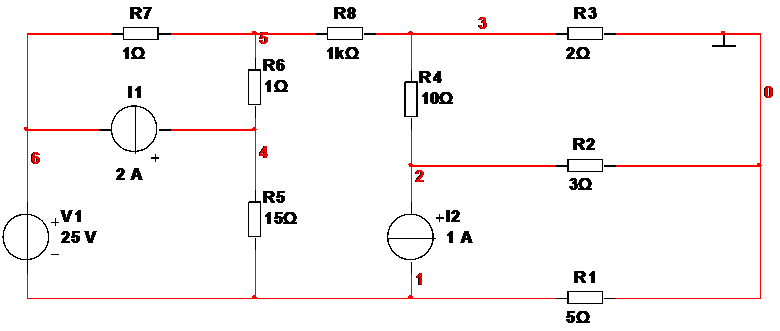
\includegraphics[scale = 0.9]{photo1.png}
    \end{center}\bigskip\bigskip\par
    Метод наложения заключается в последовательном исключении из схемы всех
    источников тока, кроме одного. В данном случае имеют место 3 частные схемы с
    генератором \textit{ЭДС} $V_1$ и генераторами тока $I_1$ и $I_2$ соответственно. Токи в ветвях
    определяются как алгебраическая сумма их составляющих от каждого источника.
    Используя полученные значения и значения сопротивления резисторов, сможем
    вычислить узловые потенциалы исходной цепи.

    \newpage

    \section{\textbf{Частная схема №1}(действует источник тока $I_1$)}
    \begin{center}
        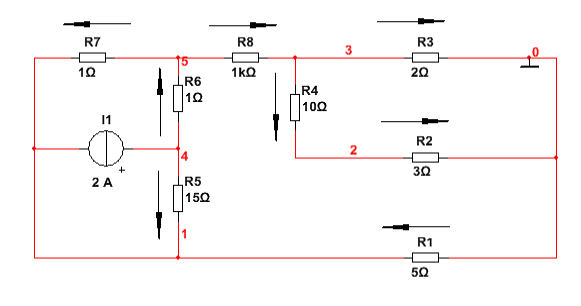
\includegraphics[scale = 1.2]{photo2.png}
    \end{center}
    \begin{itemize}
        \item После выбора направления тока можно приступать к определению токов в ветвях. Обозначение токов данной схемы будем индексировать через ``~\'~ ''.
        \item Для удобства вычислений заменим части цепи, содержащую резисторы $R_1, R_2, R_3, R_4$ и $R_8$, на участок с единственным резистором $R_{\text{экв.1}}$, имеющим сопротивление, эквивалентное исходному. Найдем это сопротивление.
    \end{itemize}
    \[ R_{\text{экв.1}} = R_8 + \frac{(R_2 + R_4)R_3}{R_2 + R_4 + R_3} + R_1 = 1000 + \frac{(3 + 10) \times 2}{3 + 10 + 2} + 5 = 1006,7333 \text{ Ом}   \]
    \begin{center}
        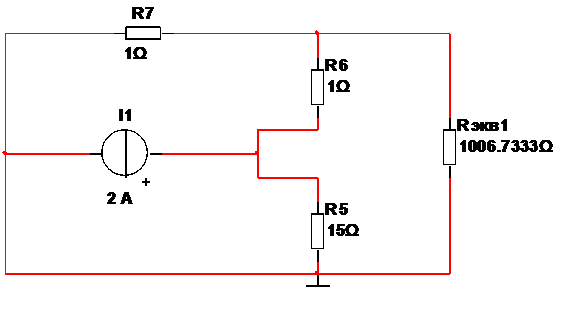
\includegraphics[scale = 1]{photo3.png}\\
        Схема 1.1
    \end{center}

    \newpage

    \begin{itemize}
        \item Данная схема (1.1) является \guillemotleftтреугольником\guillemotright. Поэтому заменим её равноценной по поведению схемой \guillemotleftзвезда\guillemotright\, с резисторами $r_1, r_2 \text{ и } r_3$
    \end{itemize}
    \begin{center}
        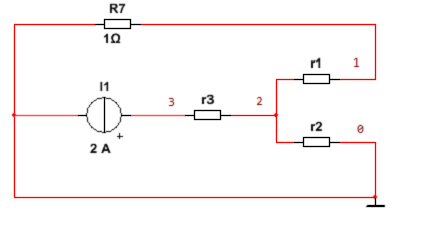
\includegraphics[scale = 1.3]{photo4.png}\\
        Схема 1.2
    \end{center}\bigskip\bigskip
    \[ r_1 = \frac{R_{6}R_{\text{экв.1}}}{R_{\text{экв.1}} + R_6 + R_5} = \frac{1 \times 1006,7333}{1006,7333 + 1 + 15} = 0,98435 \text{ Ом} \]
    \[ r_2 = \frac{R_{5}R_{\text{экв.1}}}{R_{\text{экв.1}} + R_6 + R_5} = \frac{15 \times 1006,7333}{1006,7333 + 1 + 15} = 14,7653 \text{ Ом} \]
    \[ r_3 = \frac{R_{6}R_5}{R_{\text{экв.1}} + R_6 + R_5} = \frac{1 \times 15}{1006,7333 + 1 + 15} = 0,014666 \text{ Ом} \]
    \begin{itemize}
        \item $I_{\text{г}} = I_{r_3}$ (последовательное соединение). Резисторы $r_1, r_2$ и резистор $R_7$ являются делителями тока $I_{r_3}$. Найдем $I_{R_7}$.
    \end{itemize}
    \[ I_{R_7}^\prime = I_{\text{г}}\frac{r_2}{r_1 + r_2 + R_7} = 2 \times \frac{14,7653}{0.98435 + 14,7653 + 1} = 1,76306 \text{ А} \]
    \begin{itemize}
        \item Для нахождения токов на резисторах $R_5, R_6$ и $R_{\text{экв.1}}$ необходимо найти потенциалы $\varphi_1, \varphi_3, \varphi_0$ на схеме 1.2.
    \end{itemize}
    \[ \varphi_1 = I_{R_7}^\prime R_7 = 1,76306 \times 1 = 1,76306 \text{ В} \]
    \[ \varphi_0 = 0 \text{ В} \]
    \[ \varphi_3 = I_{\text{г}}(\frac{(r_1 + R_7)r_2}{r_1 + R_7 + r_2} + r_3) = 2 \times (\frac{(0,98435 + 1) \times 14,7653}{0,98435 + 1 + 14,7653} + 0,014666) = 3,52785 \text{ В}  \]
    \begin{itemize}
        \item Найдем $I_{R_6}^\prime, I_{R_5}^\prime$ и $I_{\text{экв.1}}$
    \end{itemize}
    \[ I_{R_6}^\prime = \frac{\varphi_3 - \varphi_1}{R_6} = \frac{3,52785 - 1,76306}{1} = 1,7648 \text{ А} \]
    \[ I_{R_5}^\prime = \frac{\varphi_3 - \varphi_0}{R_5} = \frac{3,52785}{15} = 235,19 \text{ \textit{м}А} \]
    \[ I_{\text{экв.1}} = \frac{\varphi_1 - \varphi_0}{I_{\text{экв.1}}} = \frac{1,76306}{1006,7333} = 1,751 \text{ \textit{м}А} \]

    \newpage

    \begin{itemize}
        \item Так как известен ток на $R_{\text{экв.1}}$, можно найти токи на участке цепи, для которой была проведена данная замена
    \end{itemize}
    \begin{center}
        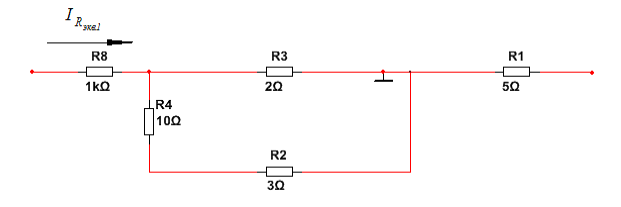
\includegraphics[scale = 1.1]{photo5.png}\\
        Схема 1.3
    \end{center}
    \[ I_{R_8}^\prime = I_{R_1}^\prime = I_{R_{\text{экв.1}}} = 1,751 \text{ \textit{м}А}  \]
    \begin{itemize}
        \item Найдем токи на оставшихся резисторах
    \end{itemize}
    \[ I_{R_3}^\prime = I_{R_{\text{экв.1}}}\frac{R_4 + R_2}{R_4 + R_2 + R_3} = 1,751 \times \frac{10 + 3}{10 + 3 + 2} = 1,517 \text{ \textit{м}А}\]
    \[ I_{R_4}^\prime = I_{R_2}^\prime = I_{R_{\text{экв.1}}}\frac{R_3}{R_4 + R_2 + R_3} = 1,751 \times \frac{2}{10 + 3 + 2} = 0,2335 \text{ \textit{м}А}\]\bigskip\bigskip\bigskip

    \section{\textbf{Частная схема №2}(действует источник тока $I_2$)}

    \begin{center}
        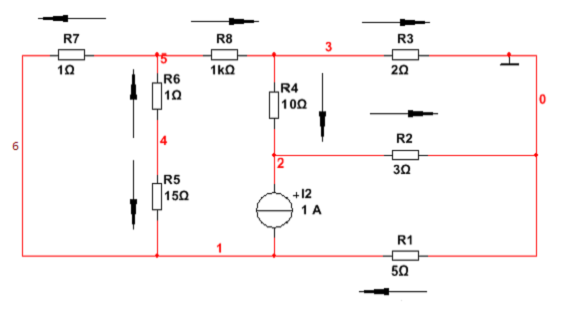
\includegraphics[scale = 1.2]{photo6.png}
    \end{center}

    \newpage

    \begin{itemize}
        \item Направление тока оставим неизменным для возможности суммировать токи на частных схемах, и таким образом получить истинные значения токов в ветвях. Обозначение токов данной схемы будем индексировать через ``~\'\'~ ''.
        \item Заменим резисторы $R_2, R_3$ и $R_4$ равноценной по поведению схемой \guillemotleftзвезда\guillemotright\, с резисторами $r_0, r_2$ и $r_3$. Найдем эти сопротивления.
    \end{itemize}
    \begin{center}
        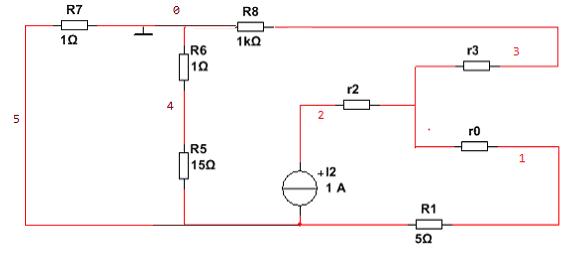
\includegraphics[scale = 1.2]{photo8.png}\\
        Схема 2.1
    \end{center}
    \[ r_0 = \frac{R_{2}R_3}{R_2 + R_3 + R_4} = \frac{3 \times 2}{3 + 2 + 10} = 0,4 \text{ Ом} \]
    \[ r_2 = \frac{R_{2}R_4}{R_2 + R_3 + R_4} = \frac{3 \times 10}{3 + 2 + 10} = 2 \text{ Ом} \]
    \[ r_3 = \frac{R_{4}R_3}{R_2 + R_3 + R_4} = \frac{10 \times 2}{3 + 2 + 10} = 1,3333 \text{ Ом} \]\bigskip
    \begin{itemize}
        \item Часть цепи с резисторами $r_3, R_5, R_6, R_7, R_8$ и часть цепи с резисторами $r_0, R_1$ являются делителями тока $I_\text{г}$. Найдем эквивалентные сопротивления для этих участвков ($R_{\text{экв.2}}$ и $R_{\text{экв.3}}$).
    \end{itemize}
    \[ R_{\text{экв.2}} = r_3 + R_8 + \frac{(R_6 + R_5)R_7}{R_6 + R_5 + R_7} = 1,3333 + 1000 + \frac{(1 + 15) \times 1}{1 + 15 + 1} = 1002,27 \text{ Ом} \]\bigskip
    \[ R_{\text{экв.3}} = r_0 + R_1 = 0,4 + 5 = 5,4 \text{ Ом} \]\bigskip
    \begin{itemize}
        \item Найдем $I_{R_1}$.
    \end{itemize}
    \[ I_{R_4}^{\prime\prime} = I_{r_0} = I_{\text{г}}\frac{R_{\text{экв.2}}}{R_{\text{экв.2}} + R_{\text{экв.3}}} = 1 \times \frac{1002,2745}{1002,2745 + 5,4} = 994,64 \text{ \textit{м}А} \]

    \newpage

    \begin{itemize}
        \item Найдем $I_{R_8}, I_{R_6}, I_{R_5}$.
    \end{itemize}
    \[ I_{R_4}^{\prime\prime} = -I_{r_3} = -I_{\text{г}}\frac{R_{\text{экв.3}}}{R_{\text{экв.2}} + R_{\text{экв.3}}} = -1 \times \frac{5,4}{1002,2745 + 5,4} = -5,36 \text{ \textit{м}А} \]
    \begin{itemize}
        \item Резистор $R_7$ и участок с резисторами $R_6$ и $R_5$ -- делители тока $I_{R_7}$. Найдем токи для данных резисторов.
    \end{itemize}
    \[ I_{R_7}^{\prime\prime} = I_{R_8}^{\prime\prime}\frac{R_6 + R_5}{R_6 + R_5 + R_7} = 0,00536 \times \frac{1 + 15}{1 + 15 + 1} = 5,044 \text{ \textit{м}А} \]
    \[ I_{R_5}^{\prime\prime} = I_{R_8}^{\prime\prime}\frac{R_7}{R_6 + R_5 + R_7} = 0,00536 \times \frac{1}{1 + 15 + 1} = 0,315 \text{ \textit{м}А} \]\bigskip
    \[ I_{R_6}^{\prime\prime} = -I_{R_5}^{\prime\prime} = -0,315 \text{ \textit{м}А} \]
    \begin{itemize}
        \item Для нахождения токов $I_{R_2}, I_{R_4}$ и $I_{R_3}$ необходимо найти потенциалы $\varphi_1, \varphi_2, \varphi_3$ на схеме №2.1.
    \end{itemize}
    \[ \varphi_1 = I_{R_1}^{\prime\prime}R_1 = 0,99464 \times 5 = 4,97 \text{ В} \]
    \[ \varphi_2 = I _{\text{г}}\frac{R_{\text{экв.2}} R_{\text{экв.3}}}{ R_{\text{экв.2}} + R_{\text{экв.3}}} + r_2 = 1 \times \frac{1002,2745 \times 5,4}{1002,2745 + 5,4} + 2 = 7,37106 \text{ В} \]
    \[ \varphi_3 = I_{R_7}^{\prime\prime}(R_{\text{экв.2}} - r_3)= 0,00536 \times (1002,2745 - 1,3333) = 5,365 \text{ В} \]
    \begin{itemize}
        \item Найдем $I_{R_2}, I_{R_4}$ и $I_{R_3}$.
    \end{itemize}
    \[ I_{R_2}^{\prime\prime} = \frac{\varphi_2 - \varphi_1}{R_2} = \frac{7,37106 - 4,97}{3} = 799 \text{ \textit{м}А} \]
    \[ I_{R_4}^{\prime\prime} = - \frac{\varphi_2 - \varphi_3}{R_4} = - \frac{7,37106 - 5,365}{10} = -200,7 \text{ \textit{м}А} \]
    \[ I_{R_3}^{\prime\prime} = \frac{\varphi_3 - \varphi_1}{R_3} = \frac{5,365 - 4,97}{2} = 195 \text{ \textit{м}А} \]\bigskip\bigskip

    \section{\textbf{Частная схема №3}(действует источник \textit{ЭДС} $V_1$)}
    \begin{center}
        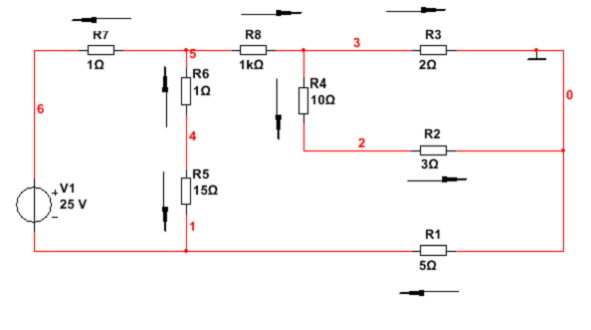
\includegraphics[scale = 1.1]{photo9.png}
    \end{center}

    \newpage

    \begin{itemize}
        \item Направление силы тока обозначим как на частной схеме №1. Обозначение токов данной схемы будем индексировать через ``~\'\'\'~ ''.
        \item Для нахождения силы тока на резисторе $R_7$ необходимо найти эквивалентное сопротивление всей цепи. Также для удобства найдем эквивалентное сопротивление участка схемы, содержащей резисторы $R_1, R_2, R_3, R_4$ и $R_8$.
    \end{itemize}
    \[ R_{\text{экв.4}} = R_8 + \frac{(R_4 + R_2)R_3}{R_2 + R_3 + R_4} + R_1 = 1000 + \frac{(10 + 3) \times 2}{10 + 3 + 2} + 5 = 1006,7333 \text{ Ом} \]
    \[ R_{\text{экв.5}} = R_7 + \frac{(R_6 + R_5)R_{\text{экв.4}}}{R_6 + R_5 + R_{\text{экв.4}}} = 1 + \frac{(1 + 15) \times 1006,7333}{1 + 15 + 1006,7333} = 16,7497 \text{ Ом} \]
    \begin{itemize}
        \item Найдем $I_{R_7}$
    \end{itemize}
    \[ I_{R_7}^{\prime\prime\prime} = - \frac{E_{\text{г}}}{R_{\text{экв.5}}} = - \frac{25}{16,7497} = - 1,4925 \text{ А} \]
    \begin{itemize}
        \item Резисторы $R_6, R_5$ и часть цепи, содержащая резисторы $R_1, R_2, R_3, R_4$ и $R_8$ соеденены параллельно и представляют собой делители тока $I_{R_7}^{\prime\prime\prime}$. Найдем токи на этих резисторах.
    \end{itemize}
    \[ I_{R_6}^{\prime\prime\prime} = I_{R_7}^{\prime\prime\prime}\frac{R_{\text{экв.4}}}{R_6 + R_5 + R_{\text{экв.4}}} = - 1,4925 \times \frac{1006,7333}{1 + 15 + 1006,7333} = - 1,469 \text{ А} \]\bigskip
    \[ I_{R_5}^{\prime\prime\prime} = - I_{R_6}^{\prime\prime\prime} = 1,469 \text{ А} \]\bigskip
    \[ I_{R_8}^{\prime\prime\prime} = I_{R_1}^{\prime\prime\prime} = - I_{R_7}^{\prime\prime\prime}\frac{R_6 + R_5}{R_6 + R_5 + R_{\text{экв.4}}} = 1,4925 \times \frac{1 + 15}{1 + 15 + 1006,7333} = 23,35 \text{\textit{ м}А} \]
    \begin{itemize}
        \item Найдем токи на $R_4, R_2$ и $R_3$ (делители тока $I_{R_8}^{\prime\prime\prime}$).
    \end{itemize}
    \[ I_{R_4}^{\prime\prime\prime} = I_{R_2}^{\prime\prime\prime} = I_{R_8}^{\prime\prime\prime}\frac{R_3}{R_2 + R_4 + R_3} = 0,02335 \times \frac{2}{3 + 10 + 2} = 3,113 \text{\textit{ м}А} \]
    \[ I_{R_{3}}^{\prime\prime\prime} = I_{R_8}^{\prime\prime\prime}\frac{R_4 + R_2}{R_2 + R_4 + R_3} = 0,02335 \times \frac{10 + 3}{3 + 10 + 2} = 20,236 \text{\textit{ м}А} \]

    \newpage

    \section{\textbf{Метод наложения}}
    \begin{center}
        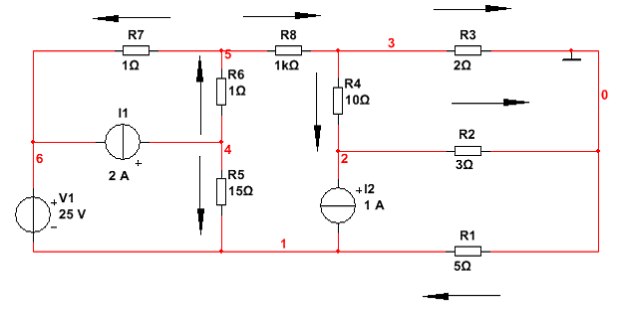
\includegraphics[scale = 1.1]{photo10.png}
    \end{center}
    \begin{itemize}
        \item Найдем истинные значения токов на резисторах путем сложения их частных значений.
    \end{itemize}
    \[ I_{R_1} = I_{R_1}^{\prime} + I_{R_1}^{\prime\prime} + I_{R_1}^{\prime\prime\prime} = 0,001751 + 0,99464 + 0,02335 = 1,019 \text{ А} \]
    \[ I_{R_2} = I_{R_2}^{\prime} + I_{R_2}^{\prime\prime} + I_{R_2}^{\prime\prime\prime} = 0,2335 + 799 + 3,113 = 802 \text{\textit{ м}А} \]
    \[ I_{R_3} = I_{R_3}^{\prime} + I_{R_3}^{\prime\prime} + I_{R_3}^{\prime\prime\prime} = 1,517 + 195 + 20,236 = 217 \text{\textit{ м}А} \]
    \[ I_{R_4} = I_{R_4}^{\prime} + I_{R_4}^{\prime\prime} + I_{R_4}^{\prime\prime\prime} = 0,2335 - 200,7 + 3,113 = - 197 \text{\textit{ м}А} \]
    \[ I_{R_5} = I_{R_5}^{\prime} + I_{R_5}^{\prime\prime} + I_{R_5}^{\prime\prime\prime} = 0,23519 + 0,000315 + 1,469 = 1,704 \text{ А} \]
    \[ I_{R_6} = I_{R_6}^{\prime} + I_{R_6}^{\prime\prime} + I_{R_6}^{\prime\prime\prime} = 1,7648 - 0,000315 - 1,469 = 295 \text{\textit{ м}А} \]
    \[ I_{R_7} = I_{R_7}^{\prime} + I_{R_7}^{\prime\prime} + I_{R_7}^{\prime\prime\prime} = 1,76306 + 0,005044 - 1,4925 = 275 \text{\textit{ м}А} \]
    \[ I_{R_8} = I_{R_8}^{\prime} + I_{R_8}^{\prime\prime} + I_{R_8}^{\prime\prime\prime} = 1,751 - 5,36 + 23,35 = 19,7 \text{\textit{ м}А} \]
    \begin{itemize}
        \item Найдем истинные значение узловых потенциалов.
    \end{itemize}
    \[ \varphi_0 = 0 \text{ В} \]
    \[ \varphi_1 = - (\varphi_1 - \varphi_0) = I_{R_1}R_1 = 1,019 \times 5 = - 5,095 \text{ В} \]
    \[ \varphi_2 = - (\varphi_0 - \varphi_2) = I_{R_2}R_2 = 0,802 \times 3 = 2,406 \text{ В} \]
    \[ \varphi_3 = - (\varphi_0 - \varphi_3) = I_{R_3}R_3 = 0,217 \times 2 = 0,434 \text{ В} \]
    \[ \varphi_4 = - (\varphi_1 - \varphi_4) = I_{R_5}R_5 = 1,704 \times 15 = 20,465 \text{ В} \]
    \[ \varphi_5 = - (\varphi_5 - \varphi_4) = I_{R_6}R_6 = 0,295 \times 1 = 20,17 \text{ В} \]
    \[ \varphi_6 = - (\varphi_6 - \varphi_5) = I_{R_7}R_7 = 0,275 \times 1 = 19,895 \text{ В} \]

    \newpage

    \section{\textbf{Проверка баланса мощностей}}
    \begin{center}
        $\sum P_{\text{пр}} = \sum P_{\text{ист}}$
    \end{center}
    \begin{itemize}
        \item Найдем ток на источнике \textit{ЭДС} $V_1$. Для этого найдем силу тока на ветви, на которой находится этот источник.
    \end{itemize}
    \textit{1) Схема 1.1}
    \[ I_{V_1}^{\prime} = I_{г_1}\frac{r_1 + R_7}{r_1 + R_7 + r_2} = 2 \times \frac{0,98435 + 1}{0,98435 + 1 + 14,7653} = 0,2369422 \text{ А} \]
    \textit{2) Схема 2.1}
    \[ I_{V_1}^{\prime\prime} = - I_{R_7}^{\prime\prime} = 0,005044 \text{ А} \]
    \textit{3) Частная схема №3}
    \[ I_{V_1}^{\prime\prime\prime} = - I_{R_7}^{\prime\prime\prime} = 1,4525 \text{ А} \]\smallskip
    \[ I_{V_1} = 0,23694422 - 0,005044 + 1,4925 = 1,7244 \text{ А} \]
    \begin{itemize}
        \item Найдем напряжения на источниках тока $I_1, I_2$.
    \end{itemize}
    \[ U_{I_1} = \varphi_4 - \varphi_6 = 0,57 \text{ B} \]
    \[ U_{I_2} = \varphi_2 - \varphi_1 = 7,5 \text{ В} \]
    \begin{itemize}
        \item Найдем мощность на всех источниках.
    \end{itemize}
    \[ \sum P_{\text{ист}} = I_{V_1}E_{V_1} + I_{1}U_{I_1} + I_{2}U_{I_2} = 1,7244 \times 25 + 2 \times 0,57 + 1 \times 7,5 = 51,75 \text{ Вт} \]
    \begin{itemize}
        \item Найдем напряжение на всех приемниках.
    \end{itemize}
    \[ \sum P_{\text{пр}} = I_{R_1}^{2}R_1 + I_{R_2}^{2}R_2 + I_{R_3}^{2}R_3 + I_{R_4}^{2}R_4 + I_{R_5}^{2}R_5 + I_{R_6}^{2}R_6 + I_{R_7}^{2}R_7 + I_{R_8}^{2}R_8 = \]
    \[= 1019^{2} \times 5 + 0,802^{2} \times 3 + 0,217^{2} \times 2 + 0,197^{2} \times 10 + 1,704^{2} \times 15 + 0,295^{2} \times 1 + 0,275^{2} \times 1 + 0,0197^{2} \times 1000 \]
    \[\sum P_{\text{пр}} = 51,7 \text{ Вт}\]\smallskip
    \text{51,75 \approx 51,7 $ \Rightarrow$ Проверка пройдена успешно с учетом погрешности.}

    \newpage

    \section{\textbf{Проверка Multisim}}
    \begin{tabular}{c c}
        \multirow{4}{*}{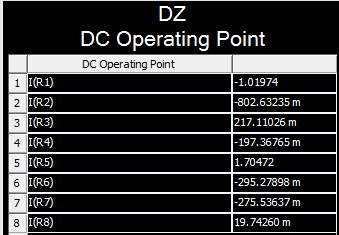
\includegraphics[scale = 1]{photo11.png}}
        & \\
        & \qquad\qquad $I_{R_1} = 1,019 \text{ А}$
        & \
        & \qquad\qquad $I_{R_2} = 802 \text{ А}$
        & \
        & \qquad\qquad $I_{R_3} = 217 \text{\textit{ м}А}$
        & \
        & \qquad\qquad $I_{R_4} = - 197 \text{\textit{ м}А}$
        & \
        & \qquad\qquad $I_{R_5} = 1,704 \text{ А}$
        & \
        & \qquad\qquad $I_{R_6} = 295 \text{\textit{ м}А}$
        & \
        & \qquad\qquad $I_{R_7} = 275 \text{\textit{ м}А}$
        & \
        & \qquad\qquad $I_{R_8} = 19,7 \text{\textit{ м}А}$
        & \\
        & \\
        & \\
        & \\
        & \\
    \end{tabular}

    \begin{tabular}{c c}
        \multirow{4}{*}{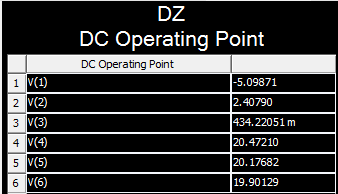
\includegraphics[scale = 1]{photo12.png}}
        & \\
        & \qquad\qquad $\varphi_0 = 0 \text{ В}$
        & \
        & \qquad\qquad $\varphi_1 = - 5,095 \text{ В}$
        & \
        & \qquad\qquad $\varphi_2 = 2,406 \text{ В}$
        & \
        & \qquad\qquad $\varphi_3 = 0,434 \text{ В}$
        & \
        & \qquad\qquad $\varphi_4 = 20,465 \text{ В}$
        & \
        & \qquad\qquad $\varphi_5 = 20,17 \text{ В}$
        & \
        & \qquad\qquad $\varphi_6 = 19,895 \text{ В}$
        & \
        & \\
        & \\
        & \\
        & \\
        & \\
    \end{tabular}

    \begin{tabular}{c c}
        \multirow{4}{*}{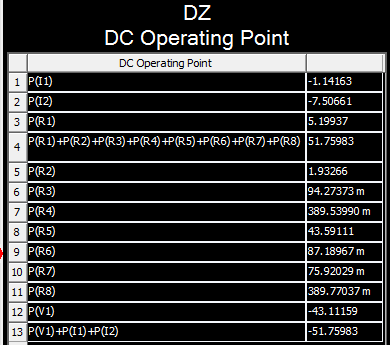
\includegraphics[scale = 0.865]{photo13.png}}
        & \\
        & \\
        & \\
        & \\
        & \\
        & \qquad\qquad $\sum P_{\text{пр}} = 51,7 \text{ Вт}$
        & \\
        & \qquad\qquad $\sum P_{\text{ист}} = 51,75 \text{ Вт}$
        & \\
        & \\
        & \\
    \end{tabular}
\end{document}